\documentclass[sigconf, nonacm]{acmart}
% Packages and macros.
\usepackage{amsmath}
\usepackage{booktabs}
\usepackage{xcolor}
\usepackage{colortbl}
\definecolor{oursblue}{HTML}{2A78D6}
\definecolor{oursorange}{HTML}{EB6834}
\definecolor{oursaqua}{HTML}{1BAF7A}
\definecolor{mutedink}{HTML}{52514E}
\definecolor{oursbg}{HTML}{E6EFFA}
\usepackage{xspace}
\usepackage{balance}
\usepackage[ruled,linesnumbered,noend]{algorithm2e}
\usepackage{graphicx}

% Long code identifiers must not overflow the narrow columns.
\setlength{\emergencystretch}{2em}

% Tight layout: no stretched columns, small caption gaps, compact lists and floats.
\raggedbottom
\usepackage[skip=0.5ex]{caption}
\setlength{\abovecaptionskip}{3pt}
\setlength{\belowcaptionskip}{3pt}
\usepackage{enumitem}
\setlist{nosep, leftmargin=*}
\setlength{\textfloatsep}{8pt plus 2pt minus 2pt}
\setlength{\floatsep}{6pt plus 2pt minus 2pt}
\setlength{\intextsep}{6pt plus 2pt minus 2pt}
\setlength{\dbltextfloatsep}{8pt plus 2pt minus 2pt}
\newcommand{\sys}{MemCommit\xspace}
\newcommand{\kw}[1]{{\ensuremath{\mathsf{#1}}}\xspace}
\newcommand{\stitle}[1]{\vspace{1.0ex}\noindent{\bf #1}}
\newcommand{\ie}{\emph{i.e.,}\xspace}
\newcommand{\eg}{\emph{e.g.,}\xspace}
\newcommand{\code}[1]{\texttt{#1}}

\usepackage{tikz}
\usetikzlibrary{positioning,arrows.meta,fit,calc}


\settopmatter{printacmref=false, printccs=false, printfolios=true}

\begin{document}

\title{MemCommit: A Transactional Memory Layer for Agents}

\author{Lam Nguyen}
\affiliation{%
  \institution{Case Western Reserve University}
  \city{Cleveland}
  \state{Ohio}
  \country{USA}}
\email{ltn18@case.edu}

\renewcommand{\shortauthors}{Nguyen}

\begin{abstract}
Agents that remember need two things at once: the full record of what
happened, so detail is never lost, and short notes of what matters, so they can
read what they know in a few lines. Most agent-memory systems keep one or the
other in a store that has no notion of a transaction, no record of where a
memory came from, and no way to take a bad one back. We present \sys, a memory
layer that treats agent memory as a database problem. Memories are immutable
and content-addressed; status and tier are a fold over an append-only log;
every memory records what it was derived from, so when a premise goes bad
everything built on it goes stale in one transaction. On this base we build
episodic sessions, derived notes at paths with a generated index and five agent
tools, an offline consolidation pass that extracts what agents did not think to
save and can be previewed and undone, and a declared memory structure that a
commit guard enforces. On a synthetic multi-session benchmark, search over the
record answers 96\% of questions from 20 words of context where the full history
needs up to 1,358; the notes reach 100\% with a perfect extractor and about 49\%
with our rule-based one, so extraction quality, not the pipeline, is the limit.
We report where the benchmark favours us and where it does not.
\end{abstract}

\keywords{agent memory, LLM agents, provenance, transactions, log-structured storage, memory consolidation}

\maketitle

\section{Introduction}
\label{sec:intro}

An agent that talks to a user for months, or a team of agents that work from
each other's output, accumulates far more than fits in a prompt. The usual
answers are a vector store of past text, a set of notes the agent writes for
itself, or both. Each leaves the same gaps. When a note was built on something
that later turns out to be wrong (a tool that was compromised, a user who
corrected themselves, a document that changed) nothing says which other notes
and answers leaned on it. When two agents write at once, nothing orders them.
When a consolidation step rewrites the notes badly, nothing takes it back. These
are the problems a database solves, and agent memory has mostly not borrowed its
answers.

\sys treats agent memory as a database problem. A memory is an immutable,
content-addressed JSON value; everything that changes about it (that it was
written, went stale, was retracted, or moved to another tier) is a record in an
append-only log, and the state of the store is a fold over that log. Every
memory names what it was \emph{derived from}, so invalidation is a graph walk:
when a premise stops holding, everything built on it goes stale, transitively,
in one transaction. Rollback is compensation, as in write-ahead logging~\cite{aries},
so nothing is erased.

On that base \sys keeps two kinds of memory. \emph{Episodic} memory is the full
record of sessions, turns, and tool calls, appended as they happen. \emph{Derived}
memory is what was learned from it: short notes at paths, with a generated index
an agent reads first, five tools it can call to save, update, delete, search, and
fetch, and an offline \emph{dreaming} pass that extracts what the agent did not
think to save, supersedes conflicting notes, merges duplicates, and splits
oversized ones. Because a note records the episodes it came from, a bad episode
takes its notes with it, and a pass can be previewed and undone. A project
declares its own memory structure once, as a schema of kinds, and a commit guard
enforces it for every writer.

\stitle{Contributions.}
\begin{itemize}
  \item A memory model that unifies a log, tiers, and provenance: status and tier are a fold over an append-only log, and invalidation and rollback follow from it (Section~\ref{sec:model}).
  \item Two tiers of memory built on that model, with an index, agent tools, an offline consolidation pass, and a declared structure, all expressed as transactions with provenance (Section~\ref{sec:tiers}).
  \item A deterministic benchmark that separates retrieval from reading and the extractor from the rest of the pipeline, with its limitations stated (Section~\ref{sec:eval}).
\end{itemize}

\noindent The library is MIT-licensed, has no runtime dependencies, and comes
with a manual and a log of the design decisions behind it.

\section{Related Work}
\label{sec:related}

\stitle{Agent memory.}
MemGPT pages information between a main context and external stores the agent
manages~\cite{memgpt}. Generative Agents keep a stream of observations and
retrieve by recency, importance, and relevance, with reflections that summarize
it~\cite{generative}; Reflexion stores verbal self-reflections after each
trial~\cite{reflexion}. MemoryOS organizes short-, mid-, and long-term stores
with heat-based promotion~\cite{memoryos}. A-MEM links notes to each other and
updates the links as notes arrive~\cite{amem}. Mem0 extracts facts and applies
add, update, delete, and no-op operations~\cite{mem0}, and Zep keeps a temporal
knowledge graph in which facts have validity intervals~\cite{zep}. \sys takes
their ideas as policies and operations on a different base: the recall score and
the summaries-as-reflections of Generative Agents, the tiers and promotion of
MemoryOS, the status operations of Mem0 as records in a log rather than updates
in place, and the temporal view of Zep as \code{as\_of(lsn)}. What these systems
do not offer together is transactions, a log with compensating rollback, and
provenance that invalidates downstream work.

\stitle{Evaluating long-term memory.}
LoCoMo~\cite{locomo} and LongMemEval~\cite{longmemeval} evaluate chat assistants
on very long conversations. We do not use them here: our benchmark is small and
synthetic, built to isolate retrieval and the extractor, and is not a substitute.

\stitle{Database ideas.}
Write-ahead logging with compensating rollback~\cite{aries}, log-structured
merge trees and the compaction they motivate~\cite{lsm}, and buffer replacement
policies (2Q~\cite{twoq}, ARC~\cite{arc}) are the direct sources of \sys's log,
its two levels of compaction, and its short-term cache and eviction policies.
Provenance as the basis for propagating changes follows the database view of
lineage~\cite{semirings}.

\section{The Memory Model}
\label{sec:model}

\stitle{Memories are values.}
A memory has a kind, a key, a body (any JSON value), the agent that wrote it, a
scope that says who may read it, an importance, and \code{derived\_from}. Its id
is a hash of all of that. Writing the same memory twice names the same memory,
and work that is redone and comes out the same restores what was there. A body
cannot change without its id changing, so tampering shows on load.

\stitle{State is a fold over a log.}
A record puts, restores, retracts, or marks stale one memory, or moves it between
tiers, inside a transaction. Status (\code{live}, \code{stale}, \code{retracted})
says whether a memory holds; tier (\code{short}, \code{mid}, \code{long},
\code{archive}) says where it sits. Neither is stored on the memory. Replaying the
log in order gives both, and \code{as\_of(lsn)} is a replay that stops early. A
transaction either commits all its records or none, and passes through guards
before the commit and observers after it. Rollback to an LSN writes the records
that return every memory to its status and tier there; the log still shows what
happened and what undid it.

\stitle{Provenance drives invalidation.}
\code{derived\_from} holds memory ids and outside references such as a document
version. Invalidating a reference marks stale every live memory reachable
through the reference index, in one transaction. A reference can also name a
\emph{read}: a memory built on ``no notes about this topic'' derives from the
query that returned nothing, and when a matching memory later goes live the work
built on the empty read goes stale. A retraction stales everything built on the
retracted memory, directly or through a read that included it.

\stitle{A declared structure.}
The core names no domain. A project declares its kinds as a schema: a JSON-schema
subset for each body, the scopes a kind may be written in, the kinds it must be
derived from, and a default tier. A commit guard rejects a write that is out of
line with its kind, for every writer in every process, and the schema is itself a
memory in the log, so \code{as\_of(lsn)} shows which structure held then. A kind
that \emph{requires} a premise (an answer derived from a question) declares
provenance together with structure.

\stitle{The cache and the database underneath.}
Short-term memory is a bounded cache in front of the log. A use counts as a hit,
a warm hit, or a miss; a missed live memory is paged back in; eviction policies
(FIFO, LRU, LFU, 2Q, ARC, a forgetting curve, a scored and a learned policy) are
pluggable. Compaction works at two levels: memory compaction folds finished
traces into long-term summaries and moves steps to the archive, and log
compaction folds each memory's history to the records that replay to the same
state, as an LSM tree rewrites sorted runs. Snapshots, hash-chain seals, a
retention policy, and a server that owns the log for agents in many processes
complete it.

\section{Two Tiers of Memory}
\label{sec:tiers}

\stitle{Episodic memory.}
A session is a trace: a root and one memory per step, each committed on its own
so that a crash keeps what was said. User and agent turns, tool calls, and tool
results are steps; a wrapper records any function's calls and results. A reply
is derived from the memories it read, so retracting one of them stales the reply.
Nothing is distilled away, so detail that a summary dropped can still be fetched.

\stitle{Derived memory.}
Notes live at paths (\code{user/alice/city}) as memories keyed by path. An update
writes a new version and marks the old one stale, and by default everything
derived from it; a delete retracts. The \emph{index} is a Markdown catalog of
every note's path, title, and first line, grouped by directory and sized to a
budget, keeping the most important and recent notes when it must cut. It is
generated on demand and meant to be injected at the start of a session. Five
tools expose the operations to a model: \code{add\_memory}, \code{update\_memory},
\code{delete\_memory}, \code{search\_memory}, and \code{fetch\_memory}. Search
spans both tiers, with relevance from a BM25 index, recency, and importance;
fetch returns a note in full, or a session as its transcript.

\stitle{Dreaming.}
Tools only save what an agent thought to save. A dreaming pass reads the sessions
that ended since the last pass, asks an extractor for the learnings in each, and
writes them as notes derived from the session and the turns they came from. It
then maintains the store: a learning whose path holds a different note replaces
it (the old note goes stale, with what was built on it), near-duplicates in a
directory are moved to the archive, and oversized notes are split into parts
derived from the original. The extractor is a function from a session to
learnings. We provide a rule-based one that needs no model, which finds stated
facts and preferences and records a successful tool sequence as a playbook; a
language model is a function with the same signature. A pass is a set of
transactions with provenance, can be previewed with a dry run, records what it
covered as a memory in the log so the next pass knows where to start, and can be
undone by rollback unless another agent has written since.

\stitle{Why transactions matter here.}
The same machinery serves all of it. A spoofed session, once retracted, stales the
notes learned from it and the replies built on those notes. A fact that changes
supersedes the old note and stales the plans built on it. A bad consolidation is
one rollback away. A declared kind refuses a malformed or orphaned write before it
lands.

\section{Evaluation}
\label{sec:eval}

We ask two questions. Does memory help an agent answer questions about earlier
conversations, and what does each tier and each writer contribute (Section~\ref{sec:memory-eval})?
And how do the cache's replacement policies compare on an agent-shaped workload
(Section~\ref{sec:policy-eval})? Both benchmarks are synthetic and deterministic, and
need no language model. They show behaviour, not real-world accuracy.

\subsection{Does memory help?}
\label{sec:memory-eval}

\stitle{Workload.}
Twenty users chat with an assistant over 8, 32, or 64 sessions each. Facts come up in
passing; one is a request to remember (``Remember that my locker code is 4412'');
40\% of users move cities later; and the rest is chatter with distractors that look
like facts (``I like long walks'', ``My friend lives in Rome''). Half the statements
are in the forms the rule-based extractor is built for (``my dog is named Rex'') and
half are paraphrases it cannot parse (``Our dog goes by the name Rex''). Afterwards
each user is asked for their current city, their dog's name, their drink, and their
locker code. We report means over three seeds.

\stitle{Reader.}
A configuration builds a context for the question from its memory, and a
recency-aware reader answers from it: the answer is the latest-mentioned of the
values the user ever gave for the attribute, and it is right if that is the current
one. This measures what memory retrieves and how clean it is, not how well a model
reads.

\stitle{Configurations.}
\emph{Full history} gives the reader everything the user said. \emph{Episodic}
searches the record and returns the best three turns. \emph{Notes} are what dreaming
extracted with the rule-based extractor, searched and returned three at a time;
\emph{notes from tools only} are those the agent saved by tool call when asked to
remember. \emph{Episodic + notes} gives three items from each tier. The \emph{oracle}
variants replace the rule-based extractor with one that parses every phrasing the
workload uses: an upper bound on extraction, which a good model-backed extractor
would approach.

\begin{table}[t]
\caption{Accuracy by sessions per user, and words of context per question at 64
sessions. Starred rows use an oracle extractor (an upper bound).}
\label{tab:memory}
\small
\setlength{\tabcolsep}{4pt}
\begin{tabular}{lcccr}
\toprule
Configuration & 8 & 32 & 64 & Words \\
\midrule
none                         & 0.000 & 0.000 & 0.000 & 0 \\
full history                 & 1.000 & 1.000 & 1.000 & 1,358 \\
episodic search              & 0.958 & 0.958 & 0.958 & 20 \\
notes from tools only        & 0.154 & 0.133 & 0.113 & 3 \\
notes (rule extractor)       & 0.492 & 0.512 & 0.487 & 15 \\
episodic + notes             & 0.942 & 0.971 & 0.958 & 35 \\
notes (oracle)*              & 1.000 & 1.000 & 1.000 & 12 \\
episodic + notes (oracle)*   & 1.000 & 1.000 & 1.000 & 33 \\
\bottomrule
\end{tabular}
\end{table}

\begin{figure*}[t]
  \centering
  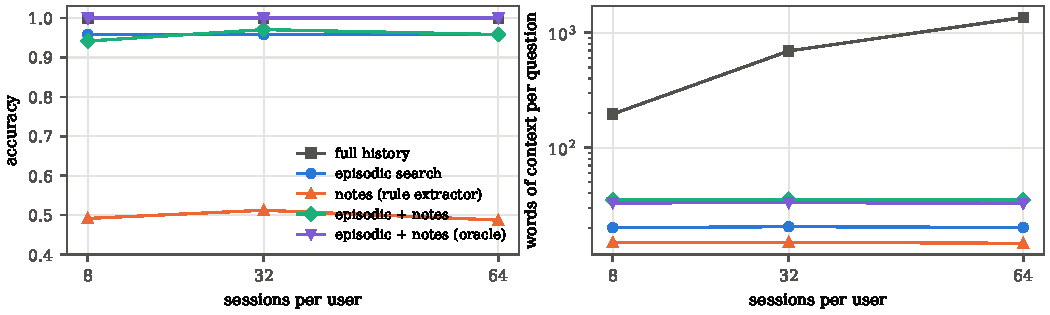
\includegraphics[width=0.8\textwidth]{fig/memory.pdf}
  \caption{Accuracy and context size as each user's history grows. The full history
  costs more with every session; search and notes read about the same amount at every
  length.}
  \label{fig:memory}
\end{figure*}

\stitle{Results.}
Table~\ref{tab:memory} and Figure~\ref{fig:memory} show four things.
(1)~\emph{The full history is not needed.} Search over the record reads about 20 words
where the full history needs 196, 694, and 1,358 as it grows, and is right 96\% of the
time.
(2)~\emph{Search alone fails on facts that change.} It is perfect on facts said once
(dog, drink, locker) and right on the city 83\% of the time, because a move often
shares few words with the question and the old statement is retrieved instead.
(3)~\emph{The notes fix that if extraction is good.} With a perfect extractor the
notes are right every time from 12 words, since the later statement supersedes the
old note and the reader sees one value. With the rule-based extractor, which parses
about half the phrasings, they are right about half the time, and the two tiers
together only match search alone. The extractor is the limit, not the pipeline.
(4)~\emph{Tools alone remember what they are told to.} Saving by tool call catches
the explicit request, and only when phrased as the agent is built to recognize it,
so accuracy is 0.11 to 0.15.

\stitle{Threats to validity.}
The workload is synthetic and small. Our first version stated every fact in the
phrasing the rule-based extractor is built for, and the notes scored 1.000; that was
circular, since both were written together, and the paraphrases are the correction.
The paraphrases were written to share a stem with the questions (``lived'' for
``live''), which favours lexical search; a paraphrase with no shared words would
defeat it and need an embedding index, which this benchmark does not test. Finally, a
recency-aware reader is not a language model.

\subsection{Eviction policies}
\label{sec:policy-eval}

We replay a synthetic agent-shaped workload (60 tasks writing 6 trace steps each,
then 472 skewed reuses of earlier memories) through the real store under each policy
and measure how often the memory an agent needs is still in working memory.
Table~\ref{tab:policy} shows hit rate at three capacities, and the log records the
policy cost at capacity 32. Every miss is a page-in and an eviction, both log records,
so cost follows quality: the forgetting curve has the best hit rate under the cap and
also writes the fewest records, 19\% fewer than FIFO. LFU and 2Q do poorly because
this workload reuses fresh trace steps often and both evict memories used only once
first. Which policy wins depends on the workload, which is why policies are pluggable
and the benchmark can replay one recorded from real agents.

\begin{table}[t]
\caption{Hit rate of working memory by capacity, and log records written at capacity 32.}
\label{tab:policy}
\small
\setlength{\tabcolsep}{4pt}
\begin{tabular}{lcccr}
\toprule
Policy & 16 & 32 & 64 & Records \\
\midrule
FIFO                & 0.506 & 0.551 & 0.602 & 1,112 \\
LRU                 & 0.642 & 0.744 & 0.828 & 930 \\
LFU                 & 0.354 & 0.460 & 0.606 & 1,198 \\
2Q                  & 0.381 & 0.481 & 0.606 & 1,178 \\
ARC                 & 0.551 & 0.663 & 0.763 & 1,006 \\
Forgetting curve    & \textbf{0.648} & \textbf{0.771} & \textbf{0.867} & \textbf{904} \\
Learned (logistic)  & 0.627 & 0.742 & 0.803 & 932 \\
\bottomrule
\end{tabular}
\end{table}

\section{Discussion and Limitations}
\label{sec:discussion}

\stitle{What the results do and do not show.}
Memory is cheap where the full history is not, and the two tiers answer different
questions: the record holds detail and facts said once, the notes hold what is
current. The case for the notes, however, rests on extraction, and our rule-based
extractor finds only about half the facts in the benchmark. A language model behind
the same signature is the largest open gain, and the benchmark's oracle rows show
what it could deliver. We have not built or measured one.

\stitle{Retrieval.}
The index matches words, not meaning. Stemming and stopword removal fixed the most
visible failures, but a paraphrase that shares no words with the query is not found.
\sys accepts any embedding function, and testing it on a workload designed to defeat
lexical search is future work.

\stitle{Scale and realism.}
Both benchmarks are synthetic, at small scale, and run in seconds. We have not
evaluated on recorded conversations or with a model as the reader, and we make no
claim about accuracy on public long-conversation benchmarks. The harness takes a
workload and a retrieval function, so both are straightforward to add.

\stitle{Design costs.}
A single log with a single writer per store keeps commits ordered and guards
meaningful, at the price of a server when agents run in many processes. Cascading
invalidation is the right default, but a frequently updated, heavily cited note
stales a lot; a flag turns it off for minor edits. Conflicts resolve by supersession,
not by judgement: the newest statement wins until someone retracts the session it came
from.

\section{Conclusion}
\label{sec:conclusion}

Agent memory is a database problem, and a log with provenance gives it transactions,
invalidation, and rollback without special cases. On that base, two tiers of memory, an
index, tools, a declared structure, and an offline consolidation pass fit together
because each is a transaction with a record of where it came from. Measured honestly
on a synthetic benchmark, the record alone is a strong baseline, and the notes are as
good as the extractor behind them.


\balance
\bibliographystyle{ACM-Reference-Format}
\bibliography{references}

\end{document}
